%%%%%%%%%%%%%%%%%%%%%%%%%%%%%%%%%%%%%%%%%
% Short Sectioned Assignment LaTeX Template Version 1.0 (5/5/12)
% This template has been downloaded from: http://www.LaTeXTemplates.com
% Original author:  Frits Wenneker (http://www.howtotex.com)
% License: CC BY-NC-SA 3.0 (http://creativecommons.org/licenses/by-nc-sa/3.0/)
%%%%%%%%%%%%%%%%%%%%%%%%%%%%%%%%%%%%%%%%%

% \documentclass[paper=a4, fontsize=11pt]{scrartcl} % A4 paper and 11pt font size
\documentclass[11pt, a4paper]{book}
\usepackage[T1]{fontenc} % Use 8-bit encoding that has 256 glyphs
\usepackage[utf8]{inputenc}
\usepackage{fourier} % Use the Adobe Utopia font for the document - comment this line to return to the LaTeX default
\usepackage{listings} % para insertar código con formato similar al editor
\usepackage[spanish, es-tabla]{babel} % Selecciona el español para palabras introducidas automáticamente, p.ej. "septiembre" en la fecha y especifica que se use la palabra Tabla en vez de Cuadro
\usepackage{url} % ,href} %para incluir URLs e hipervínculos dentro del texto (aunque hay que instalar href)
\usepackage{graphics,graphicx, float} %para incluir imágenes y colocarlas
\usepackage[gen]{eurosym} %para incluir el símbolo del euro
\usepackage{cite} %para incluir citas del archivo <nombre>.bib
\usepackage{enumerate}
\usepackage{hyperref}
\usepackage{graphicx}
\usepackage{tabularx}
\usepackage{booktabs}
\usepackage{amsmath}
\usepackage{amsfonts,amssymb}

\usepackage[table,xcdraw]{xcolor}
\hypersetup{
	colorlinks=true,	% false: boxed links; true: colored links
	linkcolor=black,	% color of internal links
	urlcolor=cyan		% color of external links
}
\renewcommand{\familydefault}{\sfdefault}
\usepackage{fancyhdr} % Custom headers and footers
\pagestyle{fancyplain} % Makes all pages in the document conform to the custom headers and footers
\fancyhead[L]{} % Empty left header
\fancyhead[C]{} % Empty center header
\fancyhead[R]{Sergio García Cabrera} % My name
\fancyfoot[L]{} % Empty left footer
\fancyfoot[C]{} % Empty center footer
\fancyfoot[R]{\thepage} % Page numbering for right footer
%\renewcommand{\headrulewidth}{0pt} % Remove header underlines
\renewcommand{\footrulewidth}{0pt} % Remove footer underlines
\setlength{\headheight}{13.6pt} % Customize the height of the header

\usepackage{titlesec, blindtext, color}
\definecolor{gray75}{gray}{0.75}
\newcommand{\hsp}{\hspace{20pt}}
\titleformat{\chapter}[hang]{\Huge\bfseries}{\thechapter\hsp\textcolor{gray75}{|}\hsp}{0pt}{\Huge\bfseries}
\setcounter{secnumdepth}{4}
\usepackage[Lenny]{fncychap}
\graphicspath{{./pictures/}}

\begin{document}

	% Plantilla portada UGR
	\begin{titlepage}
\newlength{\centeroffset}
\setlength{\centeroffset}{-0.5\oddsidemargin}
\addtolength{\centeroffset}{0.5\evensidemargin}
\thispagestyle{empty}

\noindent\hspace*{\centeroffset}\begin{minipage}{\textwidth}

\centering

\includegraphics[width=0.9\textwidth]{logos/logo_ugr.jpg}\\[1.4cm]

\textsc{ \Large TRABAJO FIN DE GRADO\\[0.2cm]}
\textsc{ GRADO EN INGENIERIA INFORMATICA}\\[1cm]

{\Huge\bfseries Título \\}
\noindent\rule[-1ex]{\textwidth}{3pt}\\[3.5ex]
{\large\bfseries Subtítulo }
\end{minipage}

\vspace{2.5cm}
\noindent\hspace*{\centeroffset}
\begin{minipage}{\textwidth}
\centering

\textbf{Autor}\\ {Estudiante}\\[2.5ex]
\textbf{Director}\\ {Tutor(a)(es)}\\[2cm]

\includegraphics[width=0.3\textwidth]{logos/etsiit_logo.png}\\[0.1cm]
\textsc{Escuela Técnica Superior de Ingenierías Informática y de Telecomunicación}\\
\textsc{---}\\
Granada, Junio de 201x
\end{minipage}
\end{titlepage}


	% Plantilla prefacio UGR
	\thispagestyle{empty}

\begin{center}
{\large\bfseries Introducción al Fuzzing, uso y estrategias de Fuzzing
para encontrar vulnerabilidades en dispositivos IoT}\\
\end{center}
\begin{center}
Sergio García Cabrera\\
\end{center}

%\vspace{0.7cm}

\vspace{0.5cm}
\noindent{\textbf{Palabras clave}: \textit{Fuzzing, IoT, Emulación, Vulnerabilidad, Sistemas empotrados,
,Black-box fuzzing, AFL++, QEMU, Open Source.}
\vspace{0.7cm}

\noindent{\textbf{Resumen}\\
Dado el creciente incremento de dispositivos conectados a internet a nuestro alrededor y la cada vez más 
sensible información que estos manejan, es una necesidad innegable el invertir una mayor cantidad de
recursos en la protección y evaluación de la seguridad de estos productos. Por desgracia, la seguridad de 
estos es en numerosas ocasiones dejada de lado debido a diferentes motivos como las 
grandes restricciones de rendimiento y de entorno normalmente asociadas a dichos dispositivos o los intentos por parte
de los fabricantes de abaratar costes de producción en productos low-cost del internet de las cosas. \\

Esta misma tendencia se puede observar respecto a la técnica del fuzzing. Aunque el fuzzing se ha consolidado 
en los últimos años como una técnica estándar en la industria del 
software gracias a su gran capacidad para encontrar fallos y vulnerabilidades, el fuzzing orientado a 
dispositivos IoT y por ende, dispositivos empotrados es un campo de investigación considerablemente 
reciente en el que aún se están dando los primeros pasos. Sumando a las causas descritas anteriormente, 
esto se debe a que aplicar técnicas de fuzzing a este tipo de dispositivos supone nuevos retos como la 
dificultad de obtener feedback sobre la ejecución de los bloques básicos de código sin disponer del código
fuente original.

En este proyecto se investigarán y aplicarán diversos enfoques y técnicas estado del arte con el fin de 
conocer el estado actual de esta novedosa rama del fuzzing orientado a dispositivos IoT.
\cleardoublepage

\begin{center}
	{\large\bfseries Introduction to Fuzzing, use cases and strategies 
	to find vulnerabilities in IoT devices}\\
\end{center}
\begin{center}
	Sergio García Cabrera\\
\end{center}
\vspace{0.5cm}
\noindent{\textbf{Keywords}: \textit{Fuzzing, IoT, Emulation, Vulnerability, Embedded systems,
,Black-box fuzzing, AFL++, QEMU, Open Source.}
\vspace{0.7cm}

\noindent{\textbf{Abstract}\\
Given the ever-increasing rise in the number of devices connected to the internet around us and the fact 
that nowadays these are made to handle more sensible information, it is clear that it has become a 
necessity to invest more time and resources in the protection and evaluation of the security of these 
products. Unfortunately, the security measures found on these are often left aside due to reasons such as 
the performance and environment constraints commonly associated with these kinds of devices or manufacturers
trying to reduce production costs of low-cost IoT devices.\\

The same trend can be observed regarding fuzzing. Even though fuzzing has consolidated as an industry 
standard thanks to its great success finding bugs and vulnerabilities in code, IoT oriented 
fuzzing and, by extension, embedded oriented fuzzing is a research field that is not nearly as mature.
Adding up to the aforementioned issues, applying fuzzing techniques to this kind of devices comes with new 
challenges such as the difficulty to get feedback about execution of basic code blocks due to the lack of 
original source code.

In this thesis, different state-of-the-art techniques and approaches will be discussed and applied in order
to learn about the current state of such a novel research field that is IoT oriented fuzzing.
\cleardoublepage

\thispagestyle{empty}

\noindent\rule[-1ex]{\textwidth}{2pt}\\[4.5ex]

D. \textbf{Gustavo Romero López}, Profesor(a) del ...

\vspace{0.5cm}

\textbf{Informo:}

\vspace{0.5cm}

Que el presente trabajo, titulado \textit{\textbf{Introducción al Fuzzing, uso y estrategias de Fuzzing
para encontrar vulnerabilidades en dispositivos IoT}},
ha sido realizado bajo mi supervisión por \textbf{Sergio García Cabrera}, y autorizo la defensa de dicho trabajo ante el tribunal
que corresponda.

\vspace{0.5cm}

Y para que conste, expiden y firman el presente informe en Granada a Junio de 2022.

\vspace{1cm}

\textbf{El/la director(a)/es: }

\vspace{5cm}

\noindent \textbf{Gustavo Romero López}

\chapter*{Agradecimientos}
Quiero agradecer a mi familia por haberme acompañado y apoyado durante todo este viaje, especialmente
en esos momentos en los que creía que no sería capaz de seguir adelante. A mis amigos y mi pareja por 
ayudarme cuando tanto necesitaba desconectar y despejarme y por último a mi tutor, Gustavo Romero López
por orientarme pacientemente cuando ni siquiera sabía cómo enfocar el TFG.





	% Índice de contenidos
	\newpage
	\tableofcontents

	% Índice de imágenes y tablas
	\newpage
	\listoffigures

	% Si hay suficientes se incluirá dicho índice
	\listoftables 
	\newpage

	% Introducción 
	\chapter{Introducción}
\label{introduccion}

\section{Motivación}
En la actualidad, podemos fácilmente apreciar cómo los fabricantes de productos de todo tipo de
ámbitos como pueden ser la medicina, la industria, la seguridad o incluso el hogar, apuestan cada vez 
más por desarrollar nuevas iteraciones de estos productos con funcionalidades comúnmente agrupadas bajo el 
adjetivo de inteligentes o ''smart''. Este nuevo paradigma de dispositivos inteligentes capaces de 
comunicarse entre sí y trabajar de forma coordinada conocido como el ''Internet de las Cosas'' o IoT por 
sus siglas en Inglés ha experimentado un crecimiento descontrolado durante la última década debido 
principalmente a los avances realizados en campos como las telecomunicaciones o el diseño de procesadores y
SoCs con una mayor potencia y menor consumo. Tal es el crecimiento que actualmente se espera que la industria del
IoT pueda alcanzar un valor económico potencial de entre 5.5 y 12.6 miles de millones de dólares para
2030 \cite{McKinsey}.
\bigskip
Dispositivos no tan novedosos como cámaras IP o routers, al igual que otros más 
propios de la última década como asistentes de voz, Smart TVs o wearables son todos ejemplos 
de dispositivos IoT que han conseguido ser una parte esencial de nuestro día a día facilitándonos
multitud de tareas. Aunque no es secreto que este tipo de dispositivos suelen basar su funcionalidad en 
la recopilación y comunicación de información que puede llegar a ser considerada sensible, es una realidad 
que los fabricantes de dichos dispositivos no están realizando una inversión suficiente en su seguridad y 
la de los datos que manejan. Un claro ejemplo de ello es el hecho de que en Europa, casi la mitad 
de dispositivos del fabricante TP-Link utiliza credenciales por defecto \cite{Deepak}, sin forzar al usuario 
a cambiarlas o incluso el gran número de estos que son puestos a la venta a día de hoy utilizando software 
considerablemente desactualizado y vulnerable como pueden ser versiones del kernel de linux publicadas hace cerca de 
diez años y ya consideradas ''End Of Life''. Problemas como los mencionados dan lugar a grandes brechas de
seguridad, que explotadas por un atacante pueden tener consecuencias desastrosas. Ejemplo de ello es 
Mirai\cite{mirai}, un malware que identificaba dispositivos IoT como routers o cámaras IP que usaran credenciales 
por defecto conocidas para infectarlos y crear una botnet que permitiera realizar ataques DDoS a gran escala.\\

Existen diversas causas que nos pueden ayudar a comprender el estado actual de la seguridad en el campo del IoT.
En primer lugar, es necesario tener en cuenta que estamos ante una industria relativamente 
joven, en claro auge y con un gran interés para todo tipo de compañías que quieren introducirse en ella diseñando 
nuevos productos pero muchas de ellas con la dificultad añadida de carecer de experiencia previa en el sector.
Esta falta de experiencia puede llevar a tomar decisiones como el realizar lanzamientos apresurados en los que la seguridad del producto no haya 
sido evaluada adecuadamente o el buscar reducir costes obviando aspectos de seguridad que puedan afectar a 
la tríada CIA (Confidentiality, Integrity, Availability) en productos de gamas low-cost donde el margen de beneficio 
es más estrecho. Respecto a vulnerabilidades software, un factor clave a tener en cuenta es la dificultad en muchos de estos 
dispositivos para que el usuario final actualice su firmware. Los altos niveles de complejidad y el gran número de dependencias del software
que es desarrollado hoy en día convierte la pregunta de \textit{¿Es este producto software vulnerable?} en algo más parecido a 
\textit{¿Cuánto tiempo tardará su seguridad en verse comprometida?} Esta realidad ejemplifica la necesidad de los fabricantes de 
proporcionar actualizaciones de firmware con parches de seguridad y de incentivar su instalación de cara al usuario, pero por 
desgracia, un gran número de sistemas empotrados o carece de actualizaciones ''Over The Air'' (OTA) o presenta una alta complejidad para 
llevar a cabo su proceso de actualización, llevando así a una baja adopción por parte de los usuarios.
Por último, cabe destacar también lo sumamente limitado que está en la mayoría de ocasiones el IoT respecto a factores como 
rendimiento, limitado por los bajos consumos requeridos, memoria, limitada por costes/tamaño del dispositivo o tiempo, limitado en sistemas de tiempo real. 
Se ha demostrado cómo para un STM32, hacer uso de un algoritmo de cifrado para las comunicaciones puede suponer 
penalizaciones de hasta 111ms\cite{performance} para cifrar y descifrar 1KB de información usando un algoritmo como AES\_CBC.\bigskip

Aplicar técnicas que pudieran ayudar a mejorar la seguridad ''automatizando'' la búsqueda de vulnerabilidades presentes en los componentes software 
de estos dispositivos sería de gran ayuda para facilitar y agilizar el proceso de identificación, análisis y corrección 
de bugs y fallos de seguridad. El fuzzing es una técnica utilizada para encontrar bugs en software mediante la ejecución de 
programas de forma repetida, haciendo uso de datos de entrada generados artificialmente a través de mutaciones aplicadas a otros
inputs. Estos inputs generados suelen distar considerablemente de los inputs para los que el software fue diseñado 
originalmente, por lo que se busca forzar a este a entrar en estados indefinidos potencialmente problemáticos. Aplicar
fuzzing a dispositivos IoT se vuelve especialmente interesante debido a que estos trabajan con grandes cantidades de inputs,
sea información en formato JSON, XML, un mensaje MQTT, se trata de inputs que provienen del exterior a través de la red y que en teoría deberían de ser validados 
de forma exhaustiva para asegurar un correcto funcionamiento incluso si la información recibida no respeta el formato o protocolo 
utilizado. Por ejemplo, aplicando fuzzing sobre un componente del firmware de un dispositivo IoT encargado de parsear información en formato JSON
se podría detectar si este presenta un comportamiento indeterminado en casos concretos como al recibir datos con caracteres especiales, lo cual
podría dar lugar a vulnerabilidades potenciales como denegación de servicio, corrupción de memoria o filtración de información. Respecto a casos reales
de vulnerabilidades críticas encontradas en dispositivos IoT a través de fuzzing podemos destacar entre otros los descubrimientos realizados por la firma 
de ciberseguridad ''Comsecuris'', que gracias a aplicar fuzzing descubrieron una vulnerabilidad en el gestor de red usado en el 
sistema operativo de los vehículos Tesla la cual permitía a un atacante realizar ejecución de código de forma remota y sin autenticar \cite{TeslaMCU}.

Cabe mencionar que emplear fuzzing orientado a IoT también presenta sus propios retos y complicaciones no tan presentes en el fuzzing tradicional. 
Ejemplos de estos retos son el disponer exclusivamente de binarios compilados para otras arquitecturas, la baja velocidad de ejecución al fuzzear o la 
dificultad de aplicar rehosting entre otros y serán discutidos a lo largo del documento.\bigskip

En resumen, el fuzzing es una técnica que ha demostrado excelentes resultados a la hora de identificar bugs 
que hubieran sido difícilmente encontrados a través de otros medios y que, aún presentando retos difíciles de abordar, resulta de especial interés en
el campo del IoT ya que ayudaría a paliar el reto de las actualizaciones de firmware en sistemas empotrados previamente mencionado, reduciendo el número de bugs con el que 
estos salen al mercado y facilitaría la mejora de los estándares de seguridad actuales de la industria. Durante este proyecto trataremos de investigar
e implementar algunos de los distintos enfoques existentes en la actualidad del fuzzing IoT orientado a código y se intentará proponer 
soluciones a los retos planteados anteriormente.

\section{Objetivos}
El objetivo principal de este proyecto, es llevar a cabo una investigación sobre el estado del arte de la aplicación de fuzzing de código en dispositivos IoT
a través de emulación, es decir, ejecutando el código a fuzzear sin requerir el hardware del dispositivo en cuestión.
Además, como objetivos complementarios a cumplir durante la realización de este proyecto se plantea lo siguiente:
\begin{itemize}
    \item Estudiar y poner en práctica los enfoques más punteros y 
    conceptos relacionados al respecto como el reversing de firmware, rehosting, emulación de sistema, binarios y de instrucciones máquina, 
    sanitizadores de memoria, black-box y grey-box fuzzing. Esto se llevará a cabo desarrollando diversas pruebas de concepto que hagan uso
    de estas tecnologías.
    \item Comparar la efectividad a la hora de identificar vulnerabilidades mediante fuzzing de los distintos enfoques que serán objeto de estudio. 
    Se tendrán en cuenta parámetros como diferencias de tiempo hasta alcanzar una misma vulnerabilidad, número de ejecuciones por segundo o estabilidad.
    \item Proporcionar un entorno de trabajo a modo de contenedor Docker que contenga todas las herramientas necesarias para llevar a cabo tareas de 
    fuzzing y emulación de dispositivos IoT (fuzzing de arquitectura cruzada). Esto no solo facilitará la reproducibilidad de las pruebas de 
    concepto desarrolladas sino que también puede ser de utilidad para todo aquel dispuesto a iniciarse en este campo. Además, se hará uso de 
    integración continua para automatizar el compilado y publicación de la imagen en DockerHub.
\end{itemize}

Con la realización de este proyecto también se plantean una serie de objetivos más personales como son el poder utilizar el conocimiento obtenido 
para colaborar con fabricantes y desarrolladores de software en la búsqueda y reporte de vulnerabilidades presentes en sus productos, además de también
aportar a la comunidad de software libre generando reportes de problemas y fallos encontrados en las herramientas utilizadas, contribuyendo así
a mejorar su calidad. 

\section{Estructura del documento}
Tras realizar una introducción al problema de la seguridad en dispositivos IoT, comentar la motivación que ha impulsado
el llevar a cabo este proyecto y definir los objetivos planteados durante el primer capítulo ''\nameref{introduccion}'', a continuación en el capítulo 2 
''\nameref{planificacion}'' se procederá a tratar cómo se ha planificado el proyecto y qué metodologías se han seguido, en el capítulo 3 ''\nameref{estado_del_arte}'' se llevará a
cabo una crítica al estado del arte del fuzzing de código IoT, además de proponer soluciones y enfoques alternativos. Más adelante en el 
capítulo 4 ''\nameref{descripcion}'' se describirá el problema que se ha planteado para a continuación analizarlo en el capítulo 5 ''\nameref{analisis}'' e implementar una solución en 
el capítulo 6 ''\nameref{implementacion}''. Por último, el capítulo 7 ''\nameref{conclusiones}'' se harán unas 
conclusiones finales tratando también los trabajos futuros que se planea llevar a cabo haciendo uso del conocimiento 
adquirido durante la realización de este proyecto.

	\chapter{Estado del arte}
\label{estado_del_arte}
Tradicionalmente, en el fuzzing orientado a dispositivos IoT no se aplicaban técnicas
específicas para este tipo de dispositivos, es decir, el principal foco de atención era el fuzzing de sus portales web a través 
de peticiones HTTP(s) con un enfoque de caja negra. Este tipo de fuzzers conocidos como fuzzers no inteligentes tratan al software como si de una caja negra se tratase, 
algo que recibe unos datos de entrada y genera otros de salida. El código que se haya alcanzado para procesar la entrada internamente no es tenido en
cuenta a la hora de modificar los inputs durante el fuzzing.

\section{Fuzzing de caja negra}
El fuzzing de caja negra sigue un flujo de ejecución simple el cual comienza con la mutación de un input válido.
A partir de ahí este input mutado es utilizado como parámetro del objetivo a fuzzear, si el 
objetivo (web, binario, etc.) produce un timeout o crashea, el fuzzer registra el input que 
ha provocado este comportamiento y si el funcionamiento del objetivo es correcto se vuelve a empezar. Dentro de los fuzzers no inteligentes hay también
distintos niveles de complejidad, algunos autores proponen fuzzers extremadamente básicos que 
llevan a cabo sus modificaciones al input de forma completamente aleatoria. Este enfoque utilizado por 
herramientas como\cite{zzuf}, sigue la filosofía que dio lugar originalmente al fuzzing en 
los años 80 de la mano de Barton Miller\cite{Miller1990}.

\subsection{Fuzzing basado en mutaciones}
Modificar inputs de forma completamente aleatoria
ejemplifica el principal problema de los fuzzers no inteligentes, la baja cobertura de código. Para conseguir encontrar 
el mayor número de fallos en el código, es necesario intentar ejecutar el mayor porcentaje de este posible. Cuando 
un input está siendo generado de manera completamente aleatoria, es bastante probable que este no cumpla con
ciertas comprobaciones que el software realice sobre el formato del input. Esto provoca que el input sea descartado 
de manera prematura en la ejecución del software y no se lleguen a alcanzar secciones críticas de código.
Con el objetivo de intentar hacer frente a este reto, otros autores proponen lo que es 
conocido como el fuzzing basado en mutaciones, donde aún aplicando todavía un enfoque de caja negra se infiere
información sobre el input original a partir de la identificación de patrones y se aplican heurísticas para generar
nuevas mutaciones. Estas heurísticas pueden ser modificables en tiempo de ejecución como hace Radamsa\cite{radamsa}
para conseguir una mayor tasa de éxito de cara a encontrar vulnerabilidades. Esta herramienta ejemplifica que incluso 
un buen fuzzer de caja negra es capaz de identificar de forma efectiva vulnerabilidades críticas en productos comerciales 
ampliamente utilizados como Cisco AnyConnect, Mozilla Firefox o Google Chrome.

\subsection{Fuzzing basado en modelos}
Otros fuzzers de caja negra categorizados como fuzzers basados en modelos o ''Generation-based fuzzers''\cite{Felderer2016} en inglés, van un paso más allá y utilizan diccionarios o modelos para solo 
mutar determinados campos de forma que se maximice el número de inputs ''válidos'' generados para la aplicación a fuzzear. Esto es de 
especial interés en aplicaciones que utilizan datos con una sintaxis especialmente compleja o verbose como HTML, SQL o XML.
Boofuzz\cite{boofuzz} es un fuzzer que implementa esta idea permitiendo al usuario crear scripts de Python en los que 
se defina un formato a seguir para el input y los campos de información que pueden ser fuzzeados sin dar lugar a inputs 
inválidos. Usando esta herramienta, el equipo de ''Security for Everyone'' descubrió un 0-day (CVE-2020-29596)\cite{securityforeveryone}
en MiniWeb HTTP server, un servidor HTTP básico orientado a dispositivos empotrados por su bajo uso de recursos.
Xiaotao et al.\cite{snipuzz} proponen ''Snipuzz'', una técnica de fuzzing de caja negra orientada a IoT en la que el fuzzer es capaz de obtener feedback 
de las respuestas que devuelve el dispositivo. La idea principal es poder deducir qué código ha sido ejecutado internamente en base a 
la respuesta obtenida al realizar una petición, aunque esto suponga depender de que el fabricante utilice mensajes de respuesta descriptivos.
Gracias a esta información adicional, ''Snipuzz'' es capaz de identificar qué rol cumple cada 
byte de un input y cómo afecta su modificación a la respuesta del dispositivo.

\subsection{Fuzzing basado en aplicaciones móviles}
Otros autores hacen frente al reto de conseguir generar inputs 
válidos a través de la invocación de métodos internos de las propias aplicaciones móviles de los fabricantes de dispositivos IoT para generar los 
inputs que enviar al dispositivo.
Basados en este planteamiento surgen ''IoTFuzzer''\cite{Chen2018} y ''DIANE''\cite{Redini2021}, dos fuzzers IoT que delegan la creación de mensajes 
a las aplicaciones para smartphone de fabricantes como TP-Link o Belkin diseñadas para gestionar remotamente los dispositivos IoT. 
Se trata de un enfoque interesante a tener en cuenta ya que estas aplicaciones siempre van a generar mensajes que respeten el formato esperado
por el dispositivo receptor. Partiendo de dicho concepto, estos fuzzers analizan automáticamente el código de las aplicaciones móvil en busca de secuencias de 
métodos que envíen mensajes al dispositivo y mediante instrumentación dinámica, ejecutan estos métodos cambiando el valor de sus parámetros. La principal diferencia 
entre ambos reside en qué componente de la aplicación móvil toman como punto de partida. ''IoTFuzzer'' parte de los métodos a nivel de interfaz de usuario de la app
para introducir la información mutada de forma similar a como lo haría un usuario real. Dicho planteamiento presenta el inconveniente de que este tipo 
de aplicaciones suelen filtrar los datos introducidos, por lo que una gran cantidad de las mutaciones serán descartadas sin siquiera salir de la aplicación.
''DIANE'' soluciona el problema tomando como punto de partida aquellos métodos que sean ejecutados después del filtrado de los inputs pero antes de
que se realice el envío del mensaje al dispositivo IoT. Por desgracia, las técnicas de fuzzing de caja negra que trabajan sobre el dispositivo IoT
directamente, ya sea haciéndole peticiones o ejecutando código en el hardware, suponen un gran sacrificio respecto a rendimiento ya que un hardware 
tan limitado como el encontrado en dispositivos empotrados nunca será capaz de aportar una alta tasa de ejecuciones/respuestas por segundo, siendo esto un 
factor clave a la hora de reducir el tiempo puede tardar un fuzzer en detectar una vulnerabilidad.

\section{Fuzzing de caja blanca}
En la búsqueda por solucionar algunos de los problemas del fuzzing de caja negra como su baja eficiencia o su limitada cobertura de código, se 
adoptan enfoques de caja blanca y caja gris. El primero gira entorno a la idea de generar binarios instrumentados a partir del código fuente original. De esta forma, un compilador 
especial inserta código adicional encargado de reportar al fuzzer qué bloques básicos de código han sido ejecutados exactamente para qué inputs.
Aunque esta es la metodología más popular para realizar fuzzing de binarios en la actualidad utilizando herramientas como AFL++\cite{afl++} o 
Honggfuzz\cite{honggfuzz}, su aplicación orientada al internet de las cosas no es viable en la mayoría de casos ya que como se comentó en 
''\nameref{introduccion}'' los componentes software utilizados en firmware IoT no suelen ser de código abierto, por lo que no pueden ser recompilados 
usando compiladores que instrumenten el código. Por suerte, AFL++ también implementa distintos modos de funcionamiento de caja gris
(QEMU\cite{qemuafl}, FRIDA\cite{frida}, Unicorn\cite{unicorn}\dots) que serán tratados a continuación.

\section{Fuzzing de caja gris}
Es la dificultad para conseguir acceso al código fuente original lo que hace que un enfoque como el fuzzing de caja gris resulte mucho más atractivo 
cuando se busca conseguir una mayor cobertura de código al fuzzear binarios de los cuales no se posee el código fuente. En este caso, los fuzzers obtienen 
feedback sobre el estado interno de la ejecución del software sin necesidad de instrumentar el código fuente original. Conseguir información que pueda ser
indicativa del estado interno de la ejecución de un software es el principal reto de los fuzzers de caja gris. 
Llevar a cabo un análisis dinámico de software de este tipo en arquitecturas más comúnmente orientadas a 
propósito general como es x86-64 no es tarea difícil, pero hacerlo sobre plataformas altamente limitadas tanto en recursos como en funcionalidad
puede suponer un reto. De esta forma surge la idea de añadir una capa de abstracción a través de emulación con soluciones basadas en QEMU\cite{qemu}
que permitan realizar instrumentación dinámica de binarios. QEMU es un eficiente emulador de código abierto capaz de correr sistemas operativos y binarios
diseñados para arquitecturas como ARM en otras completamente distintas como x86-64. Aunque en muchas ocasiones el concepto de emular software se asocia a
una gran reducción de rendimiento, es necesario tener en cuenta que un ordenador de propósito general moderno como un portátil o un sobremesa es 
considerablemente más potente que la mayoría de sistemas empotrados actuales, por lo que aún habiendo un mayor overhead en la ejecución el impacto de este queda mitigado.
Los resultados de las investigaciones llevadas a cabo por Muench et al.\cite{Muench2018} muestran cómo emulando un sistema empotrado en su totalidad 
se consigue una mejora de rendimiento sobre el hardware original.

\subsection{Técnicas de emulación}
Cuando hablamos de técnicas de emulación de sistemas empotrados, podemos aplicar la siguiente clasificación:
\begin{enumerate}[I]
    \item \textbf{User-mode emulation}: Se emula exclusivamente la ejecución del binario que resulte de interés. QEMU evita tener que emular el sistema 
    operativo al completo traduciendo las llamadas al sistema de la aplicación emulada en llamadas al sistema del host. Es por ello que usar este modo 
    solo es factible si tanto el host como el huésped comparten sistema operativo. Herramientas como Qemuafl\cite{qemuafl}, un fork de QEMU modificado para añadir 
    integración con AFL++, consiguen un mayor número de 
    ejecuciones por segundo en comparación con (II), pero por desgracia el hecho de que ciertos dispositivos hardware no estén siendo emulados puede hacer imposible 
    el correcto funcionamiento del binario. Zheng et al.\cite{Zheng2019} destacan que durante sus intentos de emular distintos 
    servidores HTTP, DNS y SSH utilizados en routers comerciales, este modo de fuzzing de AFL++ basado en QEMU fue incapaz de emular correctamente ninguno de los binarios analizados.
    \item \textbf{System-mode o Full system emulation}: Se trata de una técnica que también implementa QEMU en la cual se crea una máquina virtual que emula un 
    sistema al completo, esto incluye CPU, sistema operativo, periféricos hardware, etc. Gracias a esta técnica es posible emular software que puede resultar 
    problemático aplicando (I) debido a posibles dependencias duras sobre otros dispositivos. Un gran número de autores proponen el uso de esta técnica 
    para la ejecución de software IoT fuera de su hardware original debido a que permite alcanzar un balance entre rendimiento y estabilidad. La idea es que 
    una vez el sistema al completo es emulado, es posible fuzzear un binario del firmware aplicando el enfoque que se desee, ya sea de caja negra, gris o 
    blanca (si se dispone del código fuente). Ejemplo de uso de esta técnica de emulación es FIRMADYNE\cite{Chen2016}, un proyecto basado en QEMU\cite{qemu}
    que facilita la ejecución e instrumentación de firmware IoT a través de emulación system-mode con un kernel modificado (soporte para ARM y MIPS), además de incluir un extractor de firmware y una librería para simular una NVRAM real. Aunque se trata de un concepto interesante, diversos autores 
    han demostrado como FIRMADYNE\cite{Chen2016} fracasa a la hora de emular correctamente la mayoría de firmware IoT basado en Linux, con tasas de éxito del
    $\sim$16\%\cite{Kim2020} sobre 1124 imágenes firmware puestas a prueba pertenecientes a distintos routers y cámaras IP. Mingeun et al.\cite{Kim2020} 
    sugiere que en la mayoría de los casos, los fracasos de FIRMADYNE\cite{Chen2016} vienen dados por pequeños fallos de configuración fácilmente 
    solucionables. Es por ello que proponen FirmAE, un emulador IoT que aplica heurísticas capaces de detectar fallos de configuración propios de cada
    firmware y solucionarlos. Gracias a esto se consigue una tasa de éxito del $\sim$80\% con respecto a las mismas imágenes firmware.
    Zhang et al.\cite{Zhang2021} hacen uso de ambas herramientas durante su investigación para emular firmware IoT como paso previo a la aplicación de
    fuzzing a las interfaces web de los dispositivos.
    \item \textbf{Unicorn Engine}: Unicorn\cite{unicorn} es un framework basado en QEMU que propone un enfoque de emulación ultraligero en el que el elemento único a 
    emular es la CPU. Se diferencia de (I) en que Unicorn no realiza traducción de llamadas al sistema ni gestión de señales POSIX, solo traduce instrucciones 
    máquina de la arquitectura del huésped a instrucciones comprensibles por la CPU del host. Además, proporciona una API intuitiva que facilita 
    considerablemente operaciones necesarias para la instrumentación dinámica de binarios como lecturas/escrituras de memoria y registros, mapeos de memoria o 
    la posibilidad de definir hooks que serán ejecutados al alcanzarse ciertas direcciones de memoria. Como ya se ha comentado, AFL++ dispone de integración 
    con este framework el cual posibilita la aplicación de fuzzing sobre funcionalidades específicas de binarios complejos.\bigskip 
    
    Véase un binario que obtenga su 
    input directamente desde un dispositivo hardware como una antena de radio o un chip NFC, en lugar de fuzzear el binario al completo incluyendo todo el 
    proceso de tratamiento de señales se instrumenta dinámicamente el binario para definir un nuevo punto de entrada del código y ajustar los registros
    adecuadamente para poder así fuzzear únicamente la sección de código que nos interese. Qiling\cite{qiling} es otro framework de emulación basado en
    Unicorn\cite{unicorn} que intenta combinar las ventajas de (III) con las de (I). Esto significa poder emular binarios disponiendo de soporte 
    para llamadas al sistema, librerías dinámicas, I/O y otros conceptos de alto nivel pudiendo aplicar instrumentación dinámica a través de una API fácil 
    de usar, además de poder dejar atrás limitaciones como la necesidad de que host y huésped compartan SO.
    \item \textbf{Augmented process emulation}: Técnica propuesta por Zheng et al.\cite{Zheng2019} que implementan en su fuzzer IoT Firm-AFL. El objetivo 
    principal es combinar la emulación de binarios mediante (I) durante la mayor parte del tiempo y poder de forma dinámica cambiar a (II) si se es 
    requerido durante la ejecución.
    \item \textbf{Hardware-in-the-loop}: Utilizan tanto emulación como el hardware real del dispositivo para la ejecución de código. Para implementar esta 
    técnica se suele recurrir a algún tipo de proxy capaz de redirigir al dispositivo ciertas operaciones que tengan una fuerte dependencia en el hardware
    original mientras que la mayoría de instrucciones máquina se ejecutan en la CPU de otro sistema. Aplicar un enfoque hardware-in-the-loop aporta a costa 
    de reducir escalabilidad las ventajas de usar emulación manteniendo a su vez la alta estabilidad que proporciona usar el hardware original.
    AVATAR\cite{Zaddach2014} aplica esta técnica delegando las operaciones de I/O al hardware original mientras que el resto de la ejecución se lleva a 
    cabo mediante emulación. uAFL\cite{uAFL} lleva a cabo la ejecución del software en el hardware original y extrae del dispositivo a través de JTAG
    información de cobertura de código gracias al hardware de depuración llamado ''ARM ETM'' incluido en ciertos procesadores ARM. Dado que 
    esta información necesita de una gran cantidad de recursos para ser procesada, se extrae del dispositivo para su procesamiento y se utiliza el resultado
    para guiar el proceso de fuzzing.
\end{enumerate}

\subsection{Desinfectantes}
Más allá de la emulación, también existen otras tecnologías comúnmente utilizadas en conjunción con el fuzzing IoT como son los desinfectantes y los
''Rewriters''. En primer lugar, los desinfectantes como ASAN\cite{Serebryany2012} o MSAN\cite{Stepanov2015} son herramientas que buscan ayudar con la detección de errores de memoria mediante la instrumentación 
de código. Al instrumentar el código de una aplicación, son capaces de añadir mecanismos de protección al stack y al heap además de reemplazar funciones
de acceso a memoria como \textit{malloc} o \textit{free} con versiones propias capaces de reportar información detallada sobre la operación que está siendo 
realizada. El objetivo principal de todo esto es poder monitorizar operaciones ilegales de memoria como desbordamientos de buffers, uso de memoria después de haber sido liberada (use-after-free), fugas de memoria, etc. introduciendo el mínimo overhead posible, además de poder hacer que el binario crashee en cuanto se detecte una de estas
operaciones ilegales, incluso si durante un uso normal del software esto no hubiera sido suficiente como para afectar de forma visible su funcionamiento. 
Como es lógico, facilitar a los fuzzers la detección de errores de memoria resulta toda una ventaja pero debido a que la mayoría de desinfectantes basan su
funcionamiento en la instrumentación de código fuente, su aplicación no resulta viable para el tipo de fuzzing que nos atañe. Con el objetivo de poder 
llevar esta tecnología a binarios de código cerrado surge QASAN\cite{Fioraldi2020}, un desinfectante que consigue imitar la funcionalidad de ASAN\cite{Serebryany2012} 
mediante las capacidades de instrumentación dinámica que proporciona QEMU. Como podremos observar en \nameref{experimentos}, aplicar esta herramienta 
junto a un fuzzer puede revelar bugs de memoria que no hubieran sido descubiertos aplicando fuzzing clásico. \bigskip

\subsection{Rewriters}
Respecto a los rewriters, se tratan de herramientas que buscan instrumentar estáticamente binarios, inyectando código de instrumentación directamente en 
el binario. Aunque existen multitud de rewriters siendo desarrollados actualmente como Retrowrite\cite{Dinesh2020}, e9Patch\cite{Duck2020} o 
ZAFL\cite{Nagy2021}, es necesario tener en cuenta que se tratan de herramientas muy recientes que en muchos casos pueden introducir fallos en los binarios
instrumentados además de carecer en ocasiones de funcionalidades básicas como soporte para binarios de diferentes arquitecturas más allá de x86-64. 
Dichos problemas hacen que la tecnología no esté todavía preparada para su uso a gran escala y menos aún en el contexto de los sistemas empotrados y el 
internet de las cosas, donde la gran mayoría de dispositivos están basados en otras arquitecturas.
\bigskip

Una vez ya tratados los distintos enfoques, técnicas y herramientas presentes en el panorama actual del fuzzing IoT se nos abre un gran abanico de 
posibilidades a la hora de poner en práctica y combinar el uso de algunas de estas técnicas y herramientas para intentar conseguir detectar el mayor 
número de vulnerabilidades en software orientado a sistemas empotrados e IoT. Esto será llevado a cabo más adelante en el proyecto, donde pondremos a prueba 
conceptos como el fuzzing de caja negra, emulación system-mode y user-mode, instrumentación dinámica o los desinfectantes. Por último, antes de finalizar con
esta sección cabe destacar que, aunque el fuzzing de protocolos como Zigbee o MQTT es también una rama de investigación de gran interés en el campo del
fuzzing IoT, su discusión queda fuera del alcance de este proyecto.

\bigskip


	% Estado del arte
	% 	1. Crítica al estado del arte
	% 	2. Propuesta
	\chapter{Planificación y metodología}
\label{planificacion}

\section{Metodología utilizada}
\label{metodologia}
Aunque la realización de este proyecto no requiere en gran medida desarrollar un producto software complejo, 
se ha seguido la metodología de \textit{Desarrollo basado en Issues} (IDD por sus siglas en inglés) con el fin de agilizar y organizar el trabajo.
Se trata de una metodología similar al \textit{Desarrollo basado en Funcionalidades} en la cual la idea principal es que el 
estado actual y futuro del proyecto siempre quede reflejado en el sistema de seguimiento de issues que esté siendo utilizado.
Esta metodología presenta una serie de ventajas realmente interesantes como la modularidad que proporciona el que 
los commits y las ramas del repositorio sean autocontenidas, la granularidad gracias a que los commits y las ramas 
se centran exclusivamente en una issue actual a cerrar, además de poder llevar registro de las discusiones entre 
colaboradores con respecto a los commits realizados sobre una issue. Aunque esto último no nos atañe debido a que 
el proyecto está siendo desarrollado de forma individual, se trata de un punto positivo muy a tener en cuenta en 
entornos de desarrollo colaborativo.
El IDD también se caracteriza por seguir una filosofía DRY o ''Don't Repeat Yourself'' en 
la que se incentiva el mantener de forma estructurada, unificada y centralizada toda la información de documentación 
con respecto a cambios y planificación de desarrollo con el fin de evitar problemas de redundancia y posible
fragmentación.\bigskip

El procedimiento a seguir en esta metodología empieza por la elección de un sistema de gestión de issues. Esto se 
comentará más adelante en ''\nameref{seguimiento}''. A continuación, antes de proceder con la realización de 
cualquier tarea, se crea una issue correspondiente en la quede reflejado qué se desea hacer y cómo se tiene planteado 
hacerlo. Es buena práctica agrupar issues por hitos para tener una visión más general de estas. Una vez 
creadas la issue en cuestión y su hito correspondiente, se creará una rama en la que se llevará a cabo todo el 
desarrollo relacionado con la issue. Los commits que se realicen a las ramas deberán de contener una descripción 
explicativa de los cambios e incluir en el título una categoría y una referencia a la issue que se está tratando de solucionar. Con 
esto se busca que los commits tengan enlazada toda la información necesaria para comprender fácilmente los cambios 
realizados, es decir, que sean autocontenidos. Por último, una vez que la issue haya sido cerrada a través de un 
commit, se incorporarán los cambios de la rama temática con la rama principal.

Como es posible imaginar, esta metodología puede llegar a ser un tanto abrumadora en proyectos pequeños o poco 
complejos en los cuales puede darse el caso de que el esfuerzo de documentar en el sistema de gestión de issues 
todas las tareas a realizar puede llevar más tiempo que la realización de las tareas en sí.

Por último, comentar que para la toma de apuntes sobre la información de interés encontrada y el desarrollo de 
las pruebas de concepto se ha utilizado Joplin, una herramienta de código abierto multiplataforma que 
permite tomar notas de manera organizada en formato Markdown. El poder mantener un formato constante para los apuntes
realizados en Joplin y los README del repositorio de trabajo ha sido de gran ayuda para facilitar su traslado.

\section{Temporización}
Para realizar una estimación de la duración en días y el número de horas que pueden ocupar las distintas tareas que se desea 
llevar a cabo, se hace uso de un diagrama de Gantt en el cual quede reflejada toda esta información. Un diagrama de 
Gantt es una herramienta que tiene como objetivo ayudar en la gestión de proyectos. Suele estar compuesto por una lista 
de tareas a la izquierda y un cronograma de barras a la derecha para representar de forma visual la extensión de dichas 
tareas en el tiempo. Haciendo uso de la aplicación web \hyperlink{https://www.teamgantt.com/}{TeamGantt}, se crea el 
diagrama de la figura \ref{fig:gantt}.\bigskip
\begin{figure}[H]
    \centering{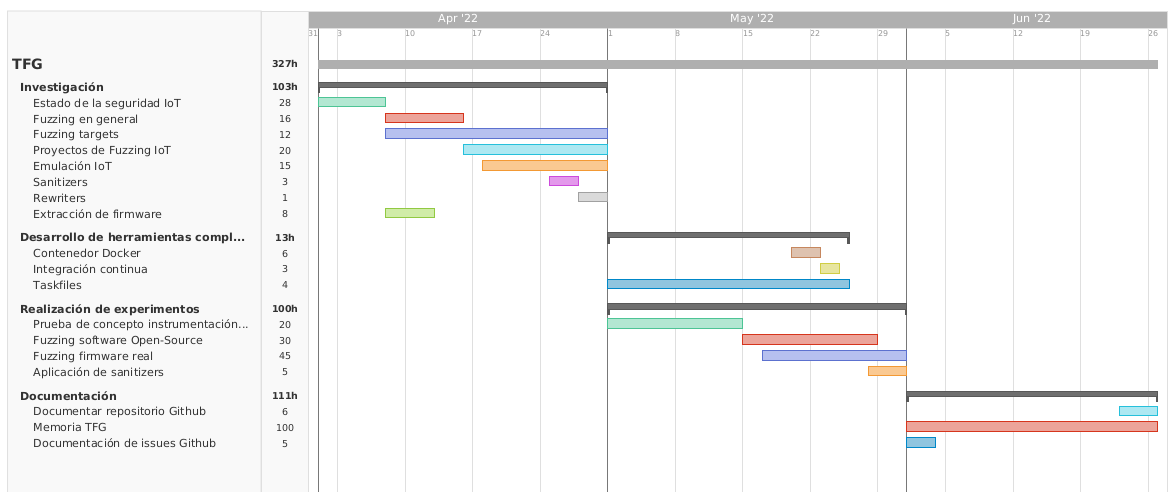
\includegraphics[scale=0.3]{Gantt.png}}
    \caption{Diagrama de Gantt con la planificación preliminar del proyecto.}
    \label{fig:gantt}
\end{figure}

La realización del proyecto se reparte en tres meses durante los cuales se plantean una serie de tareas generales a completar,
agrupadas en cuatro categorías principales, ''Investigación'', ''Desarrollo de herramientas complementarias'', ''Realización de 
experimentos'' y ''Documentación''. El siguiente listado de tareas queda reflejado en \ref{fig:gantt}:
\begin{itemize}
    \item \textbf{Investigación}: 
    \begin{itemize}
        \item \textbf{Estado de la seguridad IoT}: Como primera tarea del proyecto se ha de investigar la situación actual de la seguridad
        en el campo del internet de las cosas para tener un punto de partida.
        \item \textbf{Fuzzing en general}: Es necesario investigar el funcionamiento de la técnica del fuzzing en sí antes de proceder a 
        investigar sobre su aplicación al campo del IoT.
        \item \textbf{Fuzzing targets}: Se investigarán distintos dispositivos y sus respectivos firmwares para descubrir software de interés
        sobre el que realizar fuzzing.
        \item \textbf{Proyectos de fuzzing IoT}: Como parte del estudio del estado del arte se investigarán las distintas técnicas y herramientas 
        aplicadas actualmente en la materia.
        \item \textbf{Emulación IoT}: Dado que la emulación es un factor clave en el fuzzing IoT será necesario profundizar en las distintas 
        técnicas disponibles.
        \item \textbf{Sanitizers}: Los sanitizers o desinfectantes suelen ser utilizados para agilizar el proceso de fuzzing. Debemos de investigar cómo difiere
        su aplicación en dispositivos IoT con respecto a su uso tradicional.
        \item \textbf{Rewriters}: Investigar sobre esta nueva técnica que puede aumentar la eficiencia del fuzzing instrumentando estáticamente binarios.
        \item \textbf{Extracción de firmware}: Como paso previo a aplicar fuzzing es necesario obtener los binarios que serán objeto de
        experimento. Investigaremos la metodología actual para extraer firmware y los binarios incluidos en este.
    \end{itemize}
    \item \textbf{Desarrollo de herramientas complementarias}:
    \begin{itemize}
        \item \textbf{Contenedor Docker}: Querremos desarrollar un contenedor Docker que evite tener que lidiar con la gran cantidad de dependencias 
        y paquetes software necesarios para realizar fuzzing orientado a IoT.
        \item \textbf{Integración continua}: Se automatizará la publicación del contenedor Docker a DockerHub mediante CI/CD.
        \item \textbf{Taskfiles}: Aplicando también los conocimientos obtenidos en la asignatura de IV, se hará uso de un gestor de tareas que 
        facilitará la reproducibilidad de los experimentos. 
    \end{itemize}
    \item \textbf{Realización de experimentos}:
    \begin{itemize}
        \item \textbf{Prueba de concepto instrumentación dinámica}: Como introducción al fuzzing IoT, crearemos una prueba de concepto sobre
        un binario simple que nos permita familiarizarnos con las herramientas utilizadas y conocer las capacidades de la instrumentación dinámica.
        \item \textbf{Fuzzing software Open-Source}: Una vez se ha ganado algo de soltura con las herramientas a utilizar, se aplicará fuzzing 
        sobre un proyecto de código abierto orientado a sistemas empotrados.
        \item \textbf{Fuzzing firmware real}: Se llevará a cabo un experimento donde se aplique fuzzing a binarios extraídos del firmware de un 
        dispositivo real con el fin de identificar una vulnerabilidad conocida. 
        \item \textbf{Aplicación de sanitizers}: Para finalizar, se hará uso de desinfectantes para analizar de qué forma 
        su uso influye en el proceso de fuzzing.
    \end{itemize}
    \item \textbf{documentación}:
    \begin{itemize}
        \item \textbf{Documentar repositorio Github}: El repositorio donde llevar a cabo el control de cambios del proyecto será 
        adecuadamente documentado a través de la redacción de diversos READMEs para sus distintas secciones.
        \item \textbf{Documentación de issues Github}: Dado que van a usarse diversas herramientas de código abierto activamente 
        desarrolladas a día de hoy, será necesario documentar a través de issues en los repositorios de proyecto correspondientes
        los distintos fallos de software que se encuentren en estos durante la realización de los experimentos.
        \item \textbf{Memoria TFG}: Todo el desarrollo del proyecto de principio a fin deberá de quedar reflejado en una memoria final.
    \end{itemize}
\end{itemize}

\section{Estimación de costes}
Previamente a comenzar con el proyecto, estimaremos los costes de su realización en base a diferentes factores como el número estimado de horas necesarias, el sueldo medio de un ingeniero informático junior, los costes del hardware que necesitaremos para llevarlo a cabo o servicios necesarios
que también necesitan ser sufragados como internet o la electricidad utilizada.\bigskip

Empezamos partiendo del dato de las 327 horas estimadas en el diagrama de Gantt (figura \ref{fig:gantt}) durante 3 meses.
De esta cifra descontamos el número de horas dedicado al aprendizaje personal e investigación llevados a cabo durante el primer mes del
proyecto y utilizaremos el número de horas restantes para realizar una estimación de los costes de este proyecto. Respecto al coste de la 
mano de obra, teniendo en cuenta un 
salario medio de ingeniero informático junior de 20.000 euros brutos al año y que para llevar a cabo el proyecto se planea dedicar una media de 
4 horas diarias durante todos los días de la semana, podemos calcular un coste de $\sim13'7\euro$ la hora. Los costes de hardware se limitan al
ordenador sobre el que se va a realizar el proyecto, ya que al basar este en técnicas de emulación no va a ser requerido hardware adicional 
como podrían ser dispositivos IoT de domótica sobre los que aplicar el fuzzing. El fuzzing no requiere de ningún hardware específico para el 
ordenador con el que se va a realizar, aunque si ayuda considerablemente el tener suficiente RAM e hilos de CPU para poder aumentar el número de ejecuciones por segundo 
poniendo en marcha varias instancias en paralelo del fuzzer. Un ordenador de sobremesa como el que va a ser utilizado con 16GB de RAM, un 
Ryzen 5 3600 de 6 núcleos y 12 hilos junto con una GPU cualquiera (exclusivamente utilizada como salida de vídeo, ya que el Ryzen 5 3600 carece de GPU integrada) puede ser
conseguido por $\sim600\euro$.

Por último, el coste del servicio de internet en el lugar de trabajo actualmente es de $30\euro$ mensuales mientas 
que el coste de la luz es difícil de estimar debido a las constantes fluctuaciones en el precio de la electricidad, aunque estimaremos que 
para un un ordenador de dichas características que en el peor de los casos con la CPU trabajando al 100\% consume $\sim400W$ junto a sus 
periféricos, se produce un gasto de 1'6 KWh para 4 horas diarias de trabajo. Esto se traduce a $\sim0'37\euro$ diarios ($10'36\euro$ mensuales)
con un precio de $0'23\euro$ el KW/h. Generamos la siguiente tabla con el presupuesto estipulado:

\begin{table}[H]
    \begin{tabular}{llll}
    \rowcolor[HTML]{C0C0C0} 
    \textbf{Descripción}           & \textbf{Uds.} & \textbf{Precio/Unidad ($\euro$)} & \textbf{Total ($\euro$)} \\
    Mano de obra                   & 224           & 13'70                  & 3.068'80               \\
    Ordenador de sobremesa         & 1             & 600                    & 600                    \\
    Servicio de internet (mensual) & 2             & 30                     & 60                     \\
    Servicio de luz (mensual)      & 2             & 10'36                  & 20'72                  \\\hline
                                   &               & \textbf{Total sumado:} & 3.749'52$\euro$              
    \end{tabular}
    \caption{Presupuesto para la realización del proyecto.}
    \label{table:presupuesto}
\end{table}

Como conclusión comentar que no se trata de un presupuesto competitivo para la labor de investigación que se desea realizar. Estas tareas suelen 
ser llevadas a cabo por expertos de la materia a tratar mientras que este proyecto fue planteado para ser llevado a cabo sin experiencia previa al 
respecto con el objetivo de aprender en el proceso. Es por ello que tareas que podrían ser realizadas en menor tiempo por un investigador ya formado previamente, se prolongan 
en el tiempo con el consecuente incremento en costes.

\section{Seguimiento del desarrollo}
\label{seguimiento}
Github ha sido la plataforma de control de cambios elegida debido a que junto con Git, han sido ampliamente utilizados
en las distintas asignaturas del grado de Ingeniería Informática y ya se parte conociendo su funcionamiento y dinámica de 
trabajo. Github proporciona una funcionalidad de tablero Kanban (Figura \ref{fig:kanban}) que combinado con lo comentado en ''\nameref{metodologia}''
nos permite de un vistazo ver el estado actual de las tareas del proyecto mediante su clasificación en una serie de columnas 
definidas que agrupan las issues según si se tratan de issues por comenzar, issues en progreso, issues bloqueadas a espera 
de arreglos en software de terceros o issues completadas. Podemos observar un ejemplo de issue creada durante la realización de los 
experimentos planteados en la figura \ref{fig:issue}.
\begin{figure}[H]
    \centering{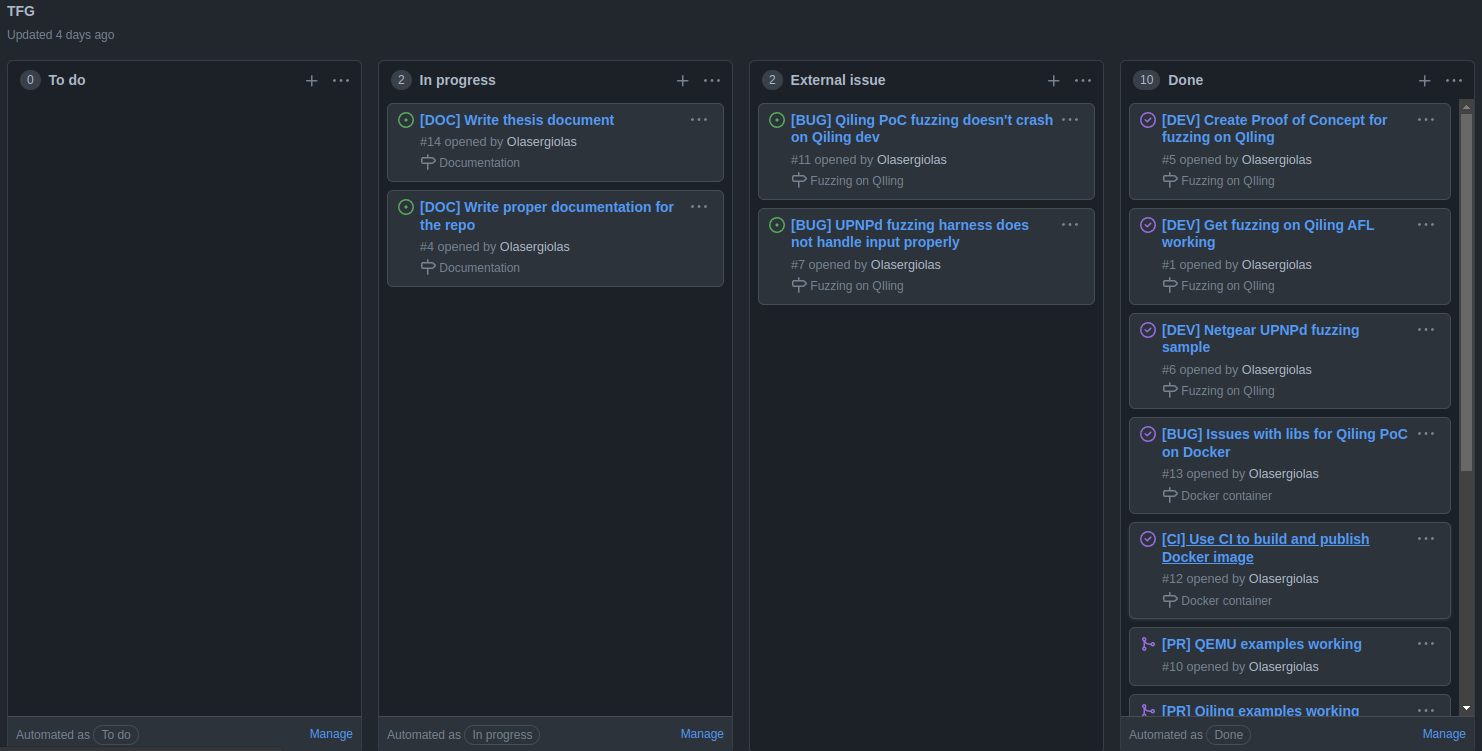
\includegraphics[scale=0.2]{kanban.png}}
    \caption{Funcionalidad de tablero Kanban de Github.}
    \label{fig:kanban}
\end{figure}

\begin{figure}[H]
    \centering{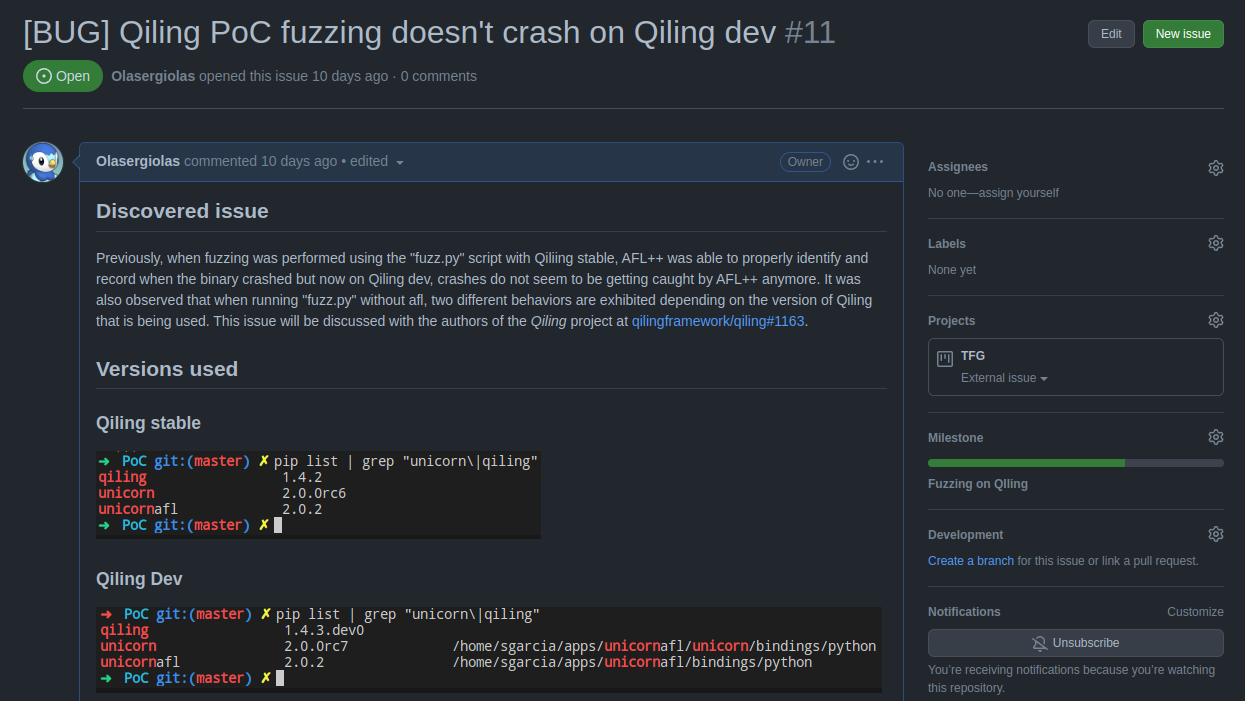
\includegraphics[scale=0.24]{issue.png}}
    \caption{Emisión de \href{https://github.com/Olasergiolas/TFG/issues/11}{informe} de error software en el repositorio del proyecto.}
    \label{fig:issue}
\end{figure}

Todo el contenido de este proyecto estará disponible públicamente en el siguiente repositorio de Github \href{https://github.com/Olasergiolas/TFG}{https://github.com/Olasergiolas/TFG}. 

	% Descripción del problema y hasta donde se llega
	\chapter{Descripción del problema}
\label{descripcion}
- Para comprender los problemas del fuzzing en IoT debemos primero tratar comprender el funcionamiento 
del fuzzing en general un poco más en profundidad ¿cómo funciona el fuzzing?.
- Para aplicar fuzzing en general necesitamos esto esto y lo otro.
- Al querer aplicarlo en IoT nos enfrentamos a X problemas (black-box, coverage, lentitud, estabilidad, 
emular de forma fiel al entorno original).
- Nombres de técnicas genéricas, sin especificar productos concretos como QEMU o Unicorn.	

	% Análisis del problema
	% 1. Análisis de requisitos
	% 2. Análisis de las soluciones
	% 3. Solucion propuesta
	% 4. Análisis de seguridad
	\chapter{Análisis del problema}
 \label{analisis}
 - Qué requisitos necesitamos cumplir
 - Analizar las posibles soluciones

	% Desarrollo bajo sprints: 
	% 	1. Permitir registros y login de usuarios
	% 	2. Desarrollo del sistema de incidencias
	% 	3. Desarrollo del sistema de denuncias administrativas y accidentes
	% 	4. Desarrollo del sistema de croquis
	%   5. Instalación de la aplicación de manera automática
	\chapter{Implementación}
\label{implementacion}

La implementación del software se ha dividido en hitos. Estos, han sido definidos en Github
y cada uno de ellos contiene un grupo de \textit{issues} que se corresponden con las distintas
mejoras que se han ido incorporando al software a lo largo de su desarrollo.\\



	% Conclusiones
	\chapter{Conclusiones y trabajos futuros}
\label{conclusiones}

	% Trabajos futuros
	
	\newpage
	\bibliography{bibliografia}
	\bibliographystyle{plain}
	
\end{document}

